\documentclass[10pt,a4paper,twocolumn]{article}

% ── Packages ──
\usepackage[utf8]{inputenc}
\usepackage[T1]{fontenc}
\usepackage{geometry}
\geometry{a4paper, margin=0.75in, top=0.9in, bottom=0.9in}
\usepackage{graphicx}
\usepackage{hyperref}
\usepackage{amsmath,amssymb}
\usepackage{booktabs}
\usepackage{float}
\usepackage{xcolor}
\usepackage{caption}
\usepackage{enumitem}
\usepackage{multicol}

\setlength{\columnsep}{0.3in}
\captionsetup{font=small, labelfont=bf}
\setlist{nosep, leftmargin=*}

% ── Title ──
\title{\vspace{-1.5em}\textbf{Hash-Based Digital Signatures:\\From Lamport OTS to Merkle Signature Schemes}\\[0.3em]
\large Applied Cryptography (CS 232) --- Project Report}
\author{Aicha Slaitane\\\texttt{aicha.slaitane@kaust.edu.sa} \and Abdullah Algethami\\\texttt{abdullah.algethami@kaust.edu.sa}}
\date{}

\begin{document}
\maketitle

% ══════════════════════════════════════════════════════════════
\begin{abstract}
\noindent
We design, implement, and evaluate a complete hash-based digital signature system in Python. Starting from the foundational Lamport One-Time Signature (OTS) scheme, we progress through Winternitz OTS (WOTS) and culminate in a full Merkle Signature Scheme (MSS) that lifts the one-time restriction. We conduct systematic benchmarks across a wide parameter space---varying the Winternitz parameter $w \in \{4,\dots,256\}$ and tree heights $h \in \{1,\dots,8\}$---to quantify the signature-size versus computation-time trade-off. Finally, we demonstrate the critical key-reuse vulnerability of Lamport signatures through a quantitative attack simulation, recovering the full 512-block secret key after only 20 reuses and validating the theoretical forgery probability $(1-2^{-k})^{256}$ against empirical data across 200 independent trials per configuration.
\end{abstract}

% ══════════════════════════════════════════════════════════════
\section{Introduction}

Digital signatures are a cornerstone of modern information security, providing authentication, integrity, and non-repudiation. Classical schemes such as RSA and ECDSA derive their security from the computational hardness of integer factorization and the discrete logarithm problem, respectively. However, Shor's algorithm~\cite{shor1994} demonstrates that a sufficiently powerful quantum computer can solve both problems in polynomial time, rendering these schemes insecure in a post-quantum world.

Hash-based signatures offer a fundamentally different security foundation. Their security rests on a single, well-studied assumption: the \emph{one-wayness} and \emph{(second-)preimage resistance} of the underlying cryptographic hash function. The best known quantum speedup against generic hash functions is Grover's algorithm, which provides only a quadratic advantage---reducing an $n$-bit hash from $2^n$ to $2^{n/2}$ security. For SHA-256, this yields approximately 128 bits of quantum security, aligning with NIST's Category-1 post-quantum requirement. This robustness is precisely why NIST standardized the hash-based scheme SLH-DSA (SPHINCS+) alongside the lattice-based ML-DSA in 2024.

In this project, we implement the fundamental building blocks that underpin modern hash-based signature standards: Lamport OTS, Winternitz OTS, and the Merkle Signature Scheme. All implementations use SHA-256 and are written in pure Python with no external cryptographic libraries. We accompany each construction with unit tests, systematic benchmarks, and a thorough security analysis of the key-reuse vulnerability inherent in OTS schemes.

% ══════════════════════════════════════════════════════════════
\section{Methods}

\subsection{Lamport One-Time Signatures}
Proposed by Lamport in 1979~\cite{lamport1979}, the scheme generates a secret key consisting of $n$ pairs of random blocks $\{(\text{SK}[i][0],\ \text{SK}[i][1])\}_{i=0}^{n-1}$, where $n$ is the hash output length in bits (256 for SHA-256) and each block is 32 bytes. The public key is the element-wise hash: $\text{PK}[i][b] = H(\text{SK}[i][b])$. To sign a message $m$, the signer computes $h = H(m)$ and reveals $\text{SK}[i][h_i]$ for each bit $h_i$. Verification rehashes each revealed block and compares against the public key. The resulting signature contains 256 blocks of 32 bytes each, totaling 8192 bytes, and the public key is twice that size (16384 bytes) since it stores both hash images per row.

\subsection{Winternitz OTS (WOTS)}
WOTS generalizes Lamport by processing the message hash in base-$w$ digits rather than individual bits. The secret key consists of $\ell = \ell_1 + \ell_2$ random blocks, where $\ell_1 = \lceil 256 / \log_2 w \rceil$ covers the message digits and $\ell_2 = \lfloor \log_2(\ell_1(w-1)) / \log_2 w \rfloor + 1$ covers a checksum. The checksum prevents forgery by digit reduction: decreasing any message digit would require increasing the checksum digits, which requires additional hash iterations the attacker cannot reverse. The public key is obtained by hashing each secret block $w-1$ times: $\text{PK}[i] = H^{w-1}(\text{SK}[i])$. To sign, each block is hashed $d_i$ times; to verify, the verifier applies $w-1-d_i$ additional hashes and checks against PK. This reduces signature size from $\ell_1 + \ell_2$ blocks (vs.\ Lamport's $2n$), but increases computation since each chain requires up to $w-1$ hash evaluations.

\subsection{Merkle Signature Scheme}
OTS schemes are inherently single-use. The Merkle tree construction~\cite{merkle1989} overcomes this by generating $N = 2^h$ independent OTS keypairs, hashing each OTS public key into a leaf node, and building a binary hash tree whose root serves as the long-term public key. A signature for the $i$-th message includes: (a) the OTS signature, (b) the OTS public key, and (c) an \emph{authentication path}---the $h$ sibling hashes along the path from leaf $i$ to the root. The verifier checks the OTS signature and reconstructs the root from the leaf using the authentication path, accepting if and only if the reconstructed root matches the published public key. A \texttt{next\_leaf} counter enforces strict one-time usage of each leaf, raising an error upon exhaustion.

% ══════════════════════════════════════════════════════════════
\section{Experimental Results}

All benchmarks were collected on a local Linux workstation using SHA-256. Timing measurements are medians over 5 independent runs.

\subsection{OTS Primitive Comparison}

We benchmarked Lamport OTS and WOTS across all power-of-two Winternitz parameters from $w=4$ to $w=256$. Table~\ref{tab:ots_full} summarizes the key generation, signing, verification times, and key/signature sizes.

\begin{table}[H]
\centering
\small
\begin{tabular}{lccccc}
\toprule
\textbf{Scheme} & \textbf{KG} & \textbf{Sign} & \textbf{Vrfy} & \textbf{Sig} & \textbf{PK} \\
 & (ms) & (ms) & (ms) & (B) & (B) \\
\midrule
Lamport     & 0.53 & 0.03 & 0.17 & 8192  & 16384 \\
WOTS $w\!=\!4$   & 0.29 & 0.15 & 0.15 & 4256  & 4256  \\
WOTS $w\!=\!8$   & 0.38 & 0.18 & 0.21 & 2880  & 2880  \\
WOTS $w\!=\!16$  & 0.56 & 0.30 & 0.28 & 2144  & 2144  \\
WOTS $w\!=\!32$  & 0.92 & 0.47 & 0.47 & 1760  & 1760  \\
WOTS $w\!=\!64$  & 1.49 & 0.68 & 0.84 & 1440  & 1440  \\
WOTS $w\!=\!128$ & 2.53 & 1.27 & 1.31 & 1248  & 1248  \\
WOTS $w\!=\!256$ & 4.47 & 2.28 & 2.29 & 1088  & 1088  \\
\bottomrule
\end{tabular}
\caption{OTS performance across Winternitz parameters. KG = KeyGen, Vrfy = Verify, Sig = signature size, PK = public key size.}
\label{tab:ots_full}
\end{table}

The Winternitz trade-off is clearly visible in both Table~\ref{tab:ots_full} and Figures~\ref{fig:ots_sig}--\ref{fig:ots_times}. As $w$ increases, signature size decreases logarithmically (Figure~\ref{fig:ots_sig}): WOTS with $w\!=\!256$ is 7.5$\times$ smaller than Lamport (1088\,B vs.\ 8192\,B). This reduction arises because each doubling of $w$ groups more bits per digit, reducing the number of hash chains $\ell_1$ by a factor proportional to $\log_2 w$. However, computation cost grows linearly with $w$ (Figure~\ref{fig:ots_times}), since each chain is $w-1$ hashes long: WOTS with $w\!=\!256$ is approximately 75$\times$ slower to sign than Lamport. Note that Lamport's signing is extremely fast (0.03\,ms) because it involves no hash computation at all---only selecting and copying precomputed blocks.

\begin{figure}[H]
\centering
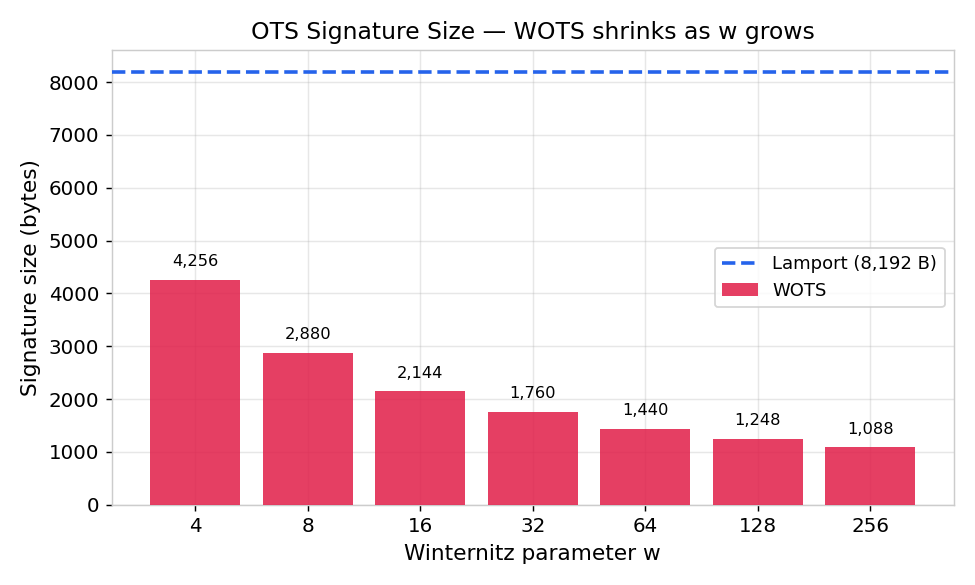
\includegraphics[width=\linewidth]{benchmarks/ots_sig_size.png}
\caption{OTS signature size vs.\ $w$. The logarithmic decrease reflects that each doubling of $w$ halves the number of base-$w$ digits needed to represent the 256-bit message hash.}
\label{fig:ots_sig}
\end{figure}

\begin{figure}[H]
\centering
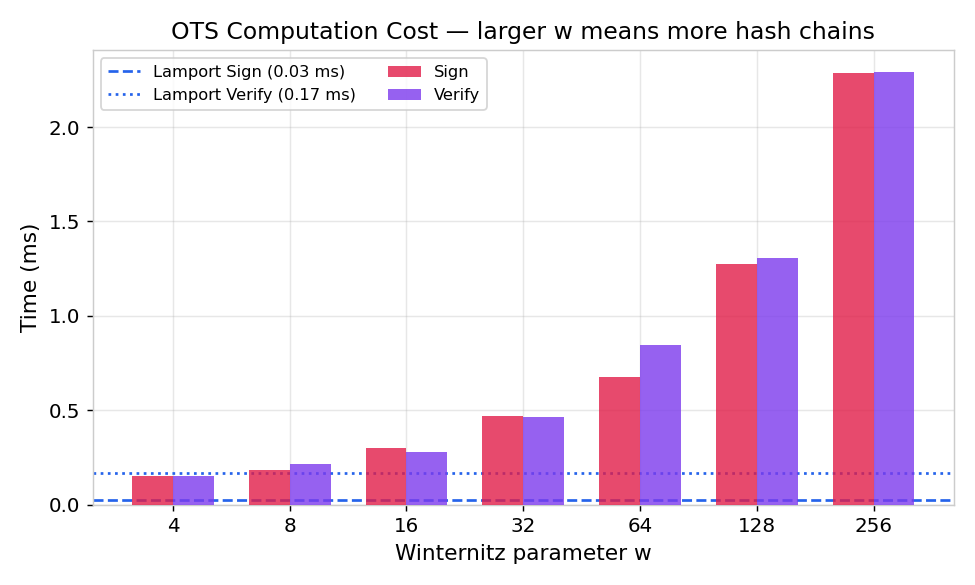
\includegraphics[width=\linewidth]{benchmarks/ots_times.png}
\caption{OTS sign and verify times vs.\ $w$. The linear growth confirms that computation is dominated by the chain length $w-1$.}
\label{fig:ots_times}
\end{figure}

\subsection{MSS Height Sweep}

Table~\ref{tab:mss_height} reports MSS performance for tree heights $h = 1$ to $8$ using both Lamport and WOTS ($w\!=\!16$) as the leaf OTS.

\begin{table}[H]
\centering
\small
\begin{tabular}{lrcccc}
\toprule
\textbf{Config} & $N$ & \textbf{KG} & \textbf{Sign} & \textbf{Vrfy} & \textbf{Sig} \\
 & & (ms) & (ms) & (ms) & (B) \\
\midrule
$h\!=\!2$, Lamp.  & 4   & 2.49   & 0.04 & 0.27 & 24644 \\
$h\!=\!4$, Lamp.  & 16  & 10.04  & 0.05 & 0.28 & 24708 \\
$h\!=\!6$, Lamp.  & 64  & 41.65  & 0.05 & 0.27 & 24772 \\
$h\!=\!8$, Lamp.  & 256 & 174.39 & 0.10 & 0.30 & 24836 \\
\midrule
$h\!=\!2$, WOTS   & 4   & 2.30   & 0.30 & 0.30 & 4356  \\
$h\!=\!4$, WOTS   & 16  & 9.08   & 0.30 & 0.30 & 4420  \\
$h\!=\!6$, WOTS   & 64  & 36.31  & 0.32 & 0.30 & 4484  \\
$h\!=\!8$, WOTS   & 256 & 144.46 & 0.31 & 0.30 & 4548  \\
\bottomrule
\end{tabular}
\caption{MSS performance vs.\ tree height ($N = 2^h$ leaves).}
\label{tab:mss_height}
\end{table}

Three key observations emerge from Table~\ref{tab:mss_height} and Figures~\ref{fig:mss_keygen}--\ref{fig:mss_sigsize}. First, as shown in Figure~\ref{fig:mss_keygen}, KeyGen scales as $O(2^h)$: going from $h\!=\!4$ to $h\!=\!8$ increases the cost by roughly 16$\times$, confirming that the dominant expense is materializing a full OTS keypair at every leaf. Second, Sign and Verify times remain effectively constant with respect to $h$ (Figures~\ref{fig:mss_sign} and~\ref{fig:mss_verify}), because the additional $h$ hash operations for the authentication path are negligible compared to the underlying OTS work. Third, signature size grows by only 32 bytes per tree level (Figure~\ref{fig:mss_sigsize})---one SHA-256 sibling hash---meaning that doubling the signing capacity ($h \to h+1$) costs a trivial 32\,B overhead per signature. Across all heights, WOTS leaves produce roughly 5.5$\times$ smaller MSS signatures than Lamport leaves ($\sim$4.5\,KB vs.\ $\sim$24.7\,KB).

\begin{figure}[H]
\centering
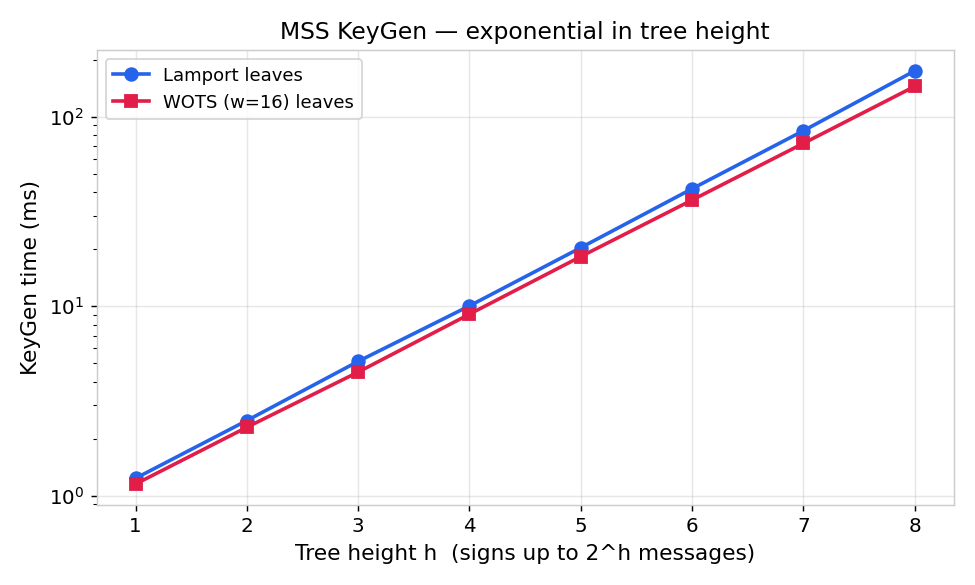
\includegraphics[width=\linewidth]{benchmarks/mss_keygen.png}
\caption{MSS KeyGen time vs.\ tree height on a log scale. The near-perfect linear trend on the log-scale confirms the $O(2^h)$ scaling.}
\label{fig:mss_keygen}
\end{figure}

\begin{figure}[H]
\centering
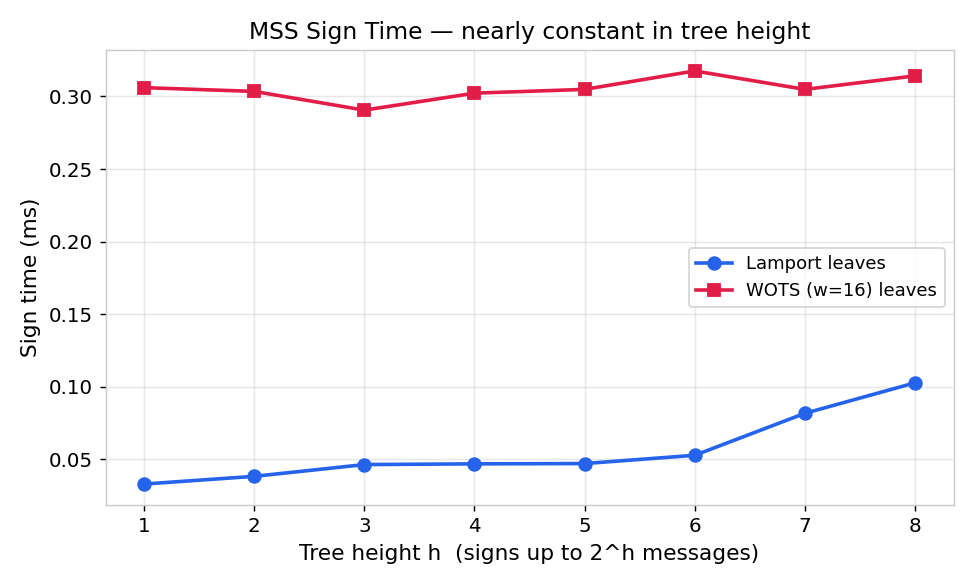
\includegraphics[width=\linewidth]{benchmarks/mss_sign.png}
\caption{MSS Sign time vs.\ height. Signing remains flat regardless of tree size, as the $h$ additional hashes are negligible next to the OTS operations.}
\label{fig:mss_sign}
\end{figure}

\begin{figure}[H]
\centering
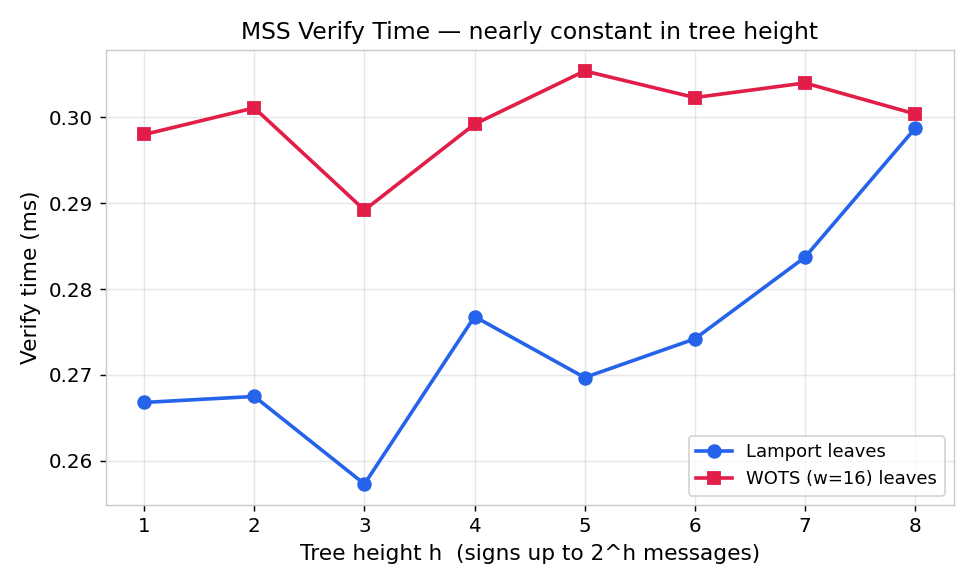
\includegraphics[width=\linewidth]{benchmarks/mss_verify.png}
\caption{MSS Verify time vs.\ height. Like signing, verification cost is dominated by the OTS check and is independent of $h$.}
\label{fig:mss_verify}
\end{figure}

\begin{figure}[H]
\centering
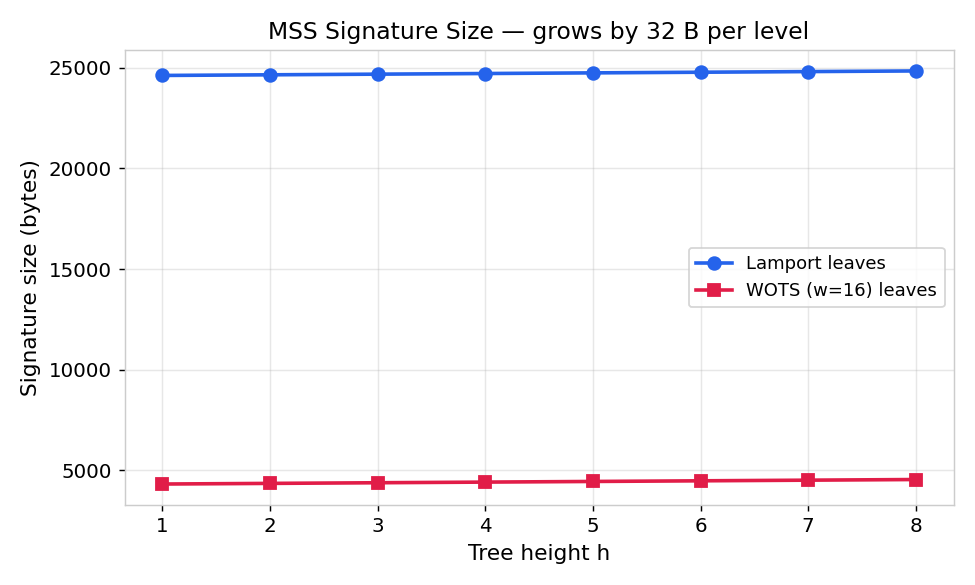
\includegraphics[width=\linewidth]{benchmarks/mss_sig_size.png}
\caption{MSS signature size vs.\ height. Growth is strictly linear at 32\,B per level, independent of the OTS backend choice.}
\label{fig:mss_sigsize}
\end{figure}

\subsection{Parameter Tuning: MSS with Varying $w$}

Fixing $h\!=\!4$ (16 leaves), we varied the WOTS parameter to study the size-vs-speed trade-off within the full MSS context (Table~\ref{tab:mss_w}). Going from $w\!=\!4$ to $w\!=\!256$ shrinks signatures by 3.7$\times$ (8644\,B to 2308\,B) but increases total computation (sign + verify) by 13$\times$. Figure~\ref{fig:mss_tradeoff} visualizes this Pareto frontier, showing the smooth and predictable nature of the trade-off curve. The ``knee'' of the curve sits near $w\!=\!16$, which is why real-world standards (XMSS, SPHINCS+) adopt this value.

\begin{table}[H]
\centering
\small
\begin{tabular}{rcccc}
\toprule
$w$ & \textbf{KG (ms)} & \textbf{Sign (ms)} & \textbf{Vrfy (ms)} & \textbf{Sig (B)} \\
\midrule
4   & 4.95  & 0.16 & 0.18 & 8644 \\
16  & 9.09  & 0.30 & 0.30 & 4420 \\
64  & 23.52 & 0.65 & 0.84 & 3012 \\
256 & 70.59 & 2.26 & 2.26 & 2308 \\
\bottomrule
\end{tabular}
\caption{MSS ($h\!=\!4$) performance vs.\ Winternitz parameter $w$.}
\label{tab:mss_w}
\end{table}

\begin{figure}[H]
\centering
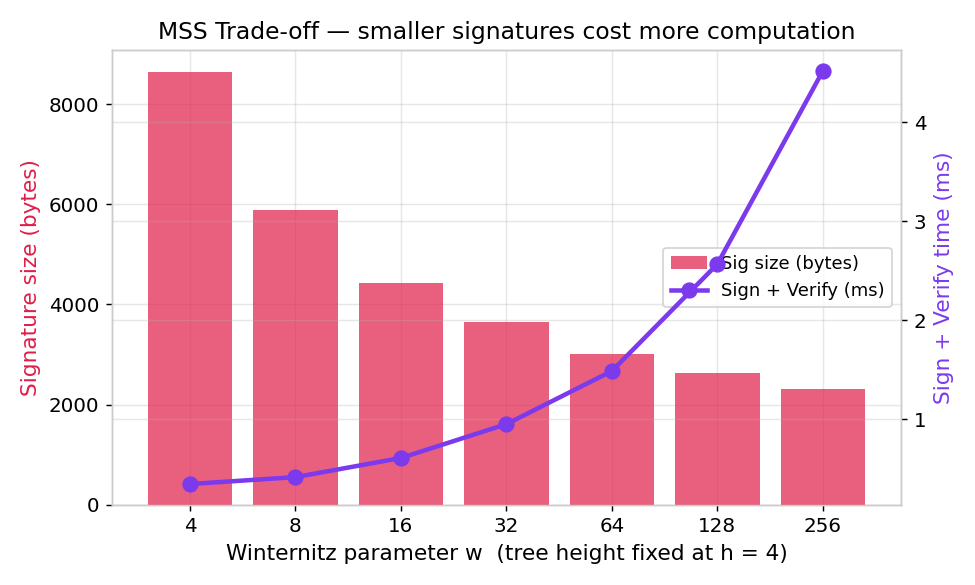
\includegraphics[width=\linewidth]{benchmarks/mss_w_tradeoff.png}
\caption{MSS size-vs-speed trade-off at $h\!=\!4$. The knee near $w\!=\!16$ marks the practical sweet spot adopted by XMSS and SPHINCS+.}
\label{fig:mss_tradeoff}
\end{figure}

Based on the complete sweep, Table~\ref{tab:recommendations} summarizes optimal parameter choices for four representative deployment priorities.

\begin{table}[H]
\centering
\small
\begin{tabular}{lcccc}
\toprule
\textbf{Priority} & \textbf{Config} & \textbf{Sig} & \textbf{S+V} & $N$ \\
\midrule
Min size    & $w\!=\!256,h\!=\!4$ & 2308\,B  & 4.52\,ms & 16  \\
Min compute & Lamp., $h\!=\!4$    & 24708\,B & 0.33\,ms & 16  \\
Balanced    & $w\!=\!16, h\!=\!5$ & 4452\,B  & 0.61\,ms & 32  \\
Max msgs    & $w\!=\!16, h\!=\!8$ & 4548\,B  & 0.61\,ms & 256 \\
\bottomrule
\end{tabular}
\caption{Recommended configurations for different priorities (S+V = Sign + Verify time, $N$ = max messages).}
\label{tab:recommendations}
\end{table}

% ══════════════════════════════════════════════════════════════
\section{Security Analysis}

\subsection{Lamport Key-Reuse Attack}

A Lamport secret key comprises $256 \times 2 = 512$ blocks. Each signature reveals exactly 256 blocks (one per row, selected by the corresponding message-hash bit). After $k$ reuses with independent random messages, the probability that a \emph{specific} block remains unrevealed is $(1/2)^k$. To forge a signature on an arbitrary target, the attacker needs all 256 blocks selected by the target's hash. The forgery probability is:
\begin{equation}
    P_{\text{forge}}(k) = \bigl(1 - 2^{-k}\bigr)^{256}
    \label{eq:forge}
\end{equation}

We verified Eq.~\eqref{eq:forge} empirically by running 200 independent trials per value of $k$, each with a fresh keypair (Table~\ref{tab:forgery}). As shown in Figure~\ref{fig:forgery}, the empirical forgery rate tracks the theoretical curve closely. After only $\sim$10 reuses, the attacker succeeds with $>$78\% probability; after 15, success is essentially certain. The attack is entirely \emph{passive}---the attacker only needs to observe legitimate signatures without any interaction with the signer.

\begin{table}[H]
\centering
\small
\begin{tabular}{rccr}
\toprule
$k$ & \textbf{Theoretical} & \textbf{Empirical} & \textbf{Exposed} \\
\midrule
1  & 0.000 & 0.000 & 50.0\% \\
4  & 0.000 & 0.000 & 93.9\% \\
6  & 0.018 & 0.030 & 98.5\% \\
8  & 0.367 & 0.385 & 99.6\% \\
10 & 0.779 & 0.835 & 99.9\% \\
12 & 0.939 & 0.950 & 100.0\% \\
14 & 0.984 & 1.000 & 100.0\% \\
20 & 1.000 & 1.000 & 100.0\% \\
\bottomrule
\end{tabular}
\caption{Forgery probability vs.\ key reuses $k$. ``Exposed'' is the average fraction of all 512 secret blocks revealed to the attacker.}
\label{tab:forgery}
\end{table}

\begin{figure}[H]
\centering
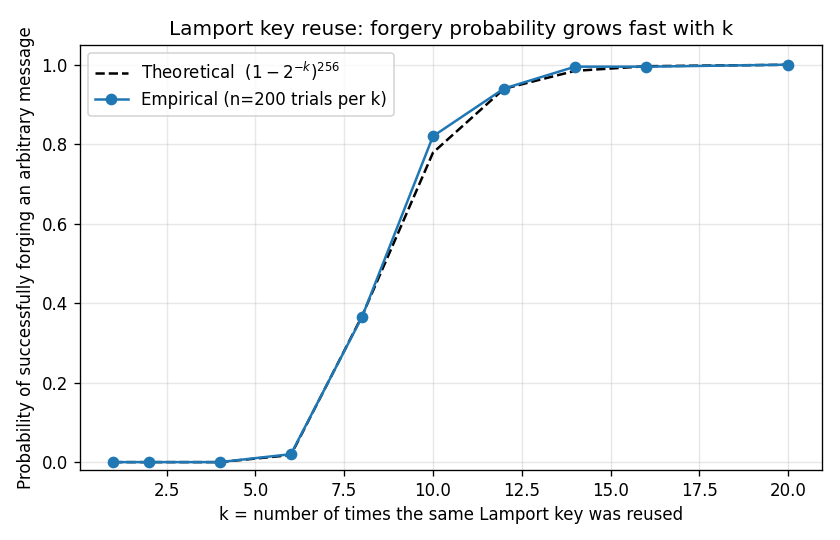
\includegraphics[width=\linewidth]{benchmarks/forgery_probability.png}
\caption{Forgery success rate vs.\ $k$. The empirical curve (200 trials per point) closely matches the theoretical prediction of Eq.~\eqref{eq:forge}, confirming the exponential convergence to certainty.}
\label{fig:forgery}
\end{figure}

Figure~\ref{fig:bits} provides a complementary view: it plots the average fraction of the 512-block secret key exposed as a function of $k$. By $k\!=\!8$, over 99.6\% of blocks are revealed, and by $k\!=\!12$ the entire key is typically exposed. This highlights that even a small number of reuses leaks nearly all secret material.

\begin{figure}[H]
\centering
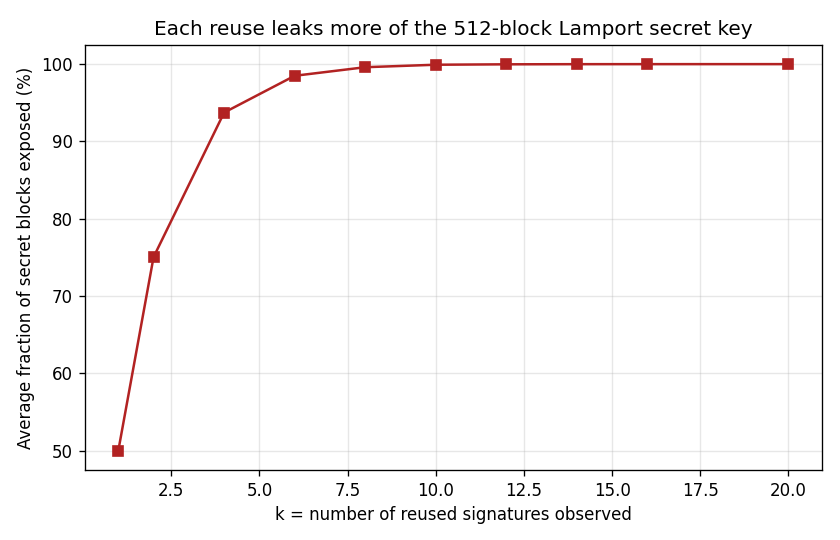
\includegraphics[width=\linewidth]{benchmarks/key_exposure.png}
\caption{Fraction of Lamport secret-key blocks exposed vs.\ reuse count $k$. Convergence to 100\% is rapid; by $k\!=\!12$ the attacker possesses the complete secret key.}
\label{fig:bits}
\end{figure}

\subsection{Full Secret Key Recovery}
We explicitly demonstrated secret-key recovery by signing 20 random messages with the same Lamport key. All 512 blocks were recovered byte-exact, as verified against the original key. The full recovered key was exported to JSON for inspection. Once in possession of the complete secret key, the attacker can forge a valid signature on \emph{any} message.

\subsection{Mitigation and Post-Quantum Security}

The key-reuse vulnerability is exactly why Lamport and WOTS are called \emph{one-time} signatures and why Merkle aggregation is mandatory for practical use. Our MSS implementation enforces one-time leaf usage via a \texttt{next\_leaf} counter that raises an error upon exhaustion. WOTS carries the same reuse risk, compounded by the checksum: forging a signature with smaller digits would require increasing the checksum digits, which requires additional hash iterations the attacker cannot compute without the secret key.

All constructions in this project derive their security solely from the preimage resistance of SHA-256. Grover's algorithm reduces the effective security from 256 bits (classical) to $\sim$128 bits (quantum), meeting NIST's Category-1 requirement. These building blocks---Lamport, WOTS, Merkle trees---are precisely the components used internally by SPHINCS+ (standardized as SLH-DSA), which adds hypertree layering to keep KeyGen practical at large heights.

% ══════════════════════════════════════════════════════════════
\section{Conclusion}

We implemented a complete hash-based signature pipeline from Lamport OTS through WOTS to the Merkle Signature Scheme, accompanied by comprehensive benchmarks and a quantitative security analysis. Our key findings are:

\begin{itemize}
    \item WOTS with $w\!=\!16$ offers the best practical balance: 3.8$\times$ smaller signatures than Lamport with sign+verify under 0.6\,ms.
    \item MSS KeyGen scales as $O(2^h)$, while signing, verification, and signature size are nearly independent of tree height.
    \item Lamport key reuse is catastrophic: after $\sim$10 reuses, forgery succeeds with $>$78\% probability; after 15 reuses, it is essentially certain.
    \item The Merkle tree construction, combined with stateful leaf tracking, fully mitigates the one-time limitation of the underlying OTS primitives.
\end{itemize}

These results confirm that hash-based signatures are a viable and well-understood path to post-quantum security, requiring only the mild assumption of hash function one-wayness.

% ══════════════════════════════════════════════════════════════
\begin{thebibliography}{9}
\bibitem{shor1994} P.~W.~Shor, ``Algorithms for quantum computation: discrete logarithms and factoring,'' \emph{Proc.\ 35th Annual Symp.\ on Foundations of Computer Science (FOCS)}, pp.~124--134, IEEE, 1994.
\bibitem{lamport1979} L.~Lamport, ``Constructing digital signatures from a one-way function,'' \emph{SRI International, Technical Report CSL-98}, 1979.
\bibitem{merkle1989} R.~C.~Merkle, ``A certified digital signature,'' \emph{Advances in Cryptology --- CRYPTO '89}, LNCS 435, pp.~218--238, Springer, 1990.
\bibitem{sphincs} D.~J.\ Bernstein et al., ``SPHINCS+: Submission to the NIST post-quantum cryptography standardization project,'' 2017.
\end{thebibliography}

\end{document}
